\documentclass[12pt]{article}

% --------------------------------------------------------------
%                       MUST HAVE PACKAGES
% --------------------------------------------------------------
\usepackage{graphicx} %handles images and other tools
\usepackage{imakeidx} %handles index file
\usepackage{hyperref} %handles hyperlinks
\usepackage[skins,theorems]{tcolorbox} %coloured boxes
\usepackage{siunitx} %SI units for ohm and others
\usepackage{systeme} %used for system of non linear equations

% --------------------------------------------------------------
%                       PROJECT SPECIFIC PACKAGES
% --------------------------------------------------------------
\usepackage{circuitikz} %circuit desing
% http://texdoc.net/texmf-dist/doc/latex/circuitikz/circuitikzmanual.pdf
\usepackage{pgfplots} %plotting


\usepackage{answers}
\usepackage{setspace}
\usepackage{enumitem}
\usepackage{multicol}
\usepackage{mathrsfs}
\usepackage[margin=1in]{geometry} 
\usepackage{amsmath,amsthm,amssymb}

%to include the folder in which images are
\graphicspath{/images/}


% short command section:
\newcommand{\N}{\mathbb{N}}
\newcommand{\Z}{\mathbb{Z}}
\newcommand{\C}{\mathbb{C}}
\newcommand{\R}{\mathbb{R}}
\newcommand{\B}{\textbf}
\newcommand{\I}{\textit}
\newcommand{\bite}{\begin{itemize}} %Begin ITEmize
\newcommand{\fite}{\end{itemize}}   %Finish ITEmize


\DeclareMathOperator{\sech}{sech}
\DeclareMathOperator{\csch}{csch}
 
\newenvironment{theorem}[2][Theorem]{\begin{trivlist}
\item[\hskip \labelsep {\bfseries #1}\hskip \labelsep {\bfseries #2.}]}{\end{trivlist}}
\newenvironment{definition}[2][Definition]{\begin{trivlist}
\item[\hskip \labelsep {\bfseries #1}\hskip \labelsep {\bfseries #2.}]}{\end{trivlist}}
\newenvironment{proposition}[2][Proposition]{\begin{trivlist}
\item[\hskip \labelsep {\bfseries #1}\hskip \labelsep {\bfseries #2.}]}{\end{trivlist}}
\newenvironment{lemma}[2][Lemma]{\begin{trivlist}
\item[\hskip \labelsep {\bfseries #1}\hskip \labelsep {\bfseries #2.}]}{\end{trivlist}}
\newenvironment{exercise}[2][Exercise]{\begin{trivlist}
\item[\hskip \labelsep {\bfseries #1}\hskip \labelsep {\bfseries #2.}]}{\end{trivlist}}
\newenvironment{solution}[2][Solution]{\begin{trivlist}
\item[\hskip \labelsep {\bfseries #1}]}{\end{trivlist}}
\newenvironment{problem}[2][Problem]{\begin{trivlist}
\item[\hskip \labelsep {\bfseries #1}\hskip \labelsep {\bfseries #2.}]}{\end{trivlist}}
\newenvironment{question}[2][Question]{\begin{trivlist}
\item[\hskip \labelsep {\bfseries #1}\hskip \labelsep {\bfseries #2.}]}{\end{trivlist}}
\newenvironment{corollary}[2][Corollary]{\begin{trivlist}
\item[\hskip \labelsep {\bfseries #1}\hskip \labelsep {\bfseries #2.}]}{\end{trivlist}}

\pgfplotsset{compat = 1.9}
\tcbset{highlight math style={enhanced,
 		colframe=red,colback=white,arc=0pt,boxrule=1pt}} %set the default box size colours
 
 \makeindex
 
\begin{document}
 
% --------------------------------------------------------------
%                         Start here
% --------------------------------------------------------------
 
 
\title{Introduction to Electronics:\\
theory, formulas and utilities}
\author{Tommaso Polloni\\
and }
 
 The very first idea is to make this document a learning tool for git, latex and, of course, of Electronics. A primary goal is to maintain English as its unique language.
\maketitle
\tableofcontents

\section{Semiconductors} \index{Semiconductors}
Semiconductors are material with an electrical conductivity value falling between that of a conductor and an insulator.
An important property of semiconductors is that, during a temperature increment, their resistance decreases.
Common semiconductors material are:
\begin{itemize}
	\item \index{Silicon}Silicon, Si. Z (i.e. atomic number) = 14. IV ($14^{th}$) group.
	\item Germanium, Ge. Atomic number = 32. IV ($14^{th}$) group
	\item Gallium Arsenide, GaAs, a compound of Gallium and Arsenic.
\end{itemize}
Another important characteristic of semiconductors is that there are two charge carriers available, holes and electrons.

 
\subsection{Semiconductors: a nuclear approach}
In 1913 Niehls Bohr \index{Nihels Bohr} proposed a model of atom in which \I{quantization of the angular momentum} \index{angular momentum} explained some interesting results regarding the light emitted by Hydrogen atoms heated. This model is very useful to explain the internal structure of atoms and can tell us something even about Silicon. A neutral Silicon atom possesses 14 protons and many electrons.
\begin{itemize}
	\item the first 10 of them lies in the first two energy level: they fit perfectly around the nucleus and  are generally not involved in chemical reactions (because of the very high amount of energy necessary to "interact" with them).
	\item the remaining 4 electrons are called \textit{valence electrons}\index{valence electrons} and are at higher energy levels. They are involved in the \textit{covalent bond}.
\end{itemize}
When temperature is near at the absolute zero ($-273^o C$) the Silicon atoms assume a crystal form in which every \textit{valence electron} is shared with the nearest 4 atoms of Silicon with a covalent bond: in this circumstance Silicon act as an \textbf{insulator}.
At higher temperatures, (i. e. furnishing energy to the atom) covalent bounds can break. 
\subsubsection{Electrons and Holes}
When the break happens, an electron \I{jumps} from valence band to conduction band and a hole is generated. The conduction-band electron is now a \B{charge carrier} and the atom it left is a charged positively (cation). 
\subsubsection{Valence and conduction bands}
Without the necessary energy, electrons remain under the \I{Fermi level}, in a zone called \I{Valence Band}. when the \I{jump} occurs, electrons step over the \I{Fermi level} and stay in the \I{conduction band}. In the conduction band charge carrier have less constraints and can easily move in the crystalline lattice, depending on the intensity of the electro-magnetic field.
\subsubsection{Silicon properties}
\bite
	\item The amount of charge carriers in a $cm^3$ (i.e. electrons in the conduction band) at ambient temperature $n = 10^{10} cm^{-3}$. It is reasonably a little number compared to the global amount of atoms in a Silicon $cm^3$ ($5 \cdot 10^{22}$). [Think that if atoms were people on earth, only 7 people would result a cation with the loss of their electron]. 
	\item It is compatible with $SiO_2$ and $Al$
\fite

\subsection{Doping}
The doping process consists in significantly change the number of \textit{electrons }or \textit{holes} in a semiconductor.
This result is achieved inserting atoms of the doping element in the crystalline arrangement of the doped.
\subsubsection{Utilities and numbers}
\begin{itemize}
	\item $N_{d} \approxeq 10^{12} : 10^{20} cm^{-3}$ number of donors
	\item $p 	[\dfrac{electrons}{cm^3}]$ number of holes 
	\item $n 	[\dfrac{electrons}{cm^3}]$ number of electrons 
\end{itemize}
Remember that:
\begin{itemize}
	\item n-doping leaves free electron in conduction band and is obtained by inserting DONORS atoms of $Phosphorus$, or other elements from the V$^{th}$ group.
	\item p-doping creates holes in the lattice structure and is obtained by inserting ACCEPTORS atoms of $Boron$, or other elements from the III$^{th}$ group. 
\end{itemize}
\subsubsection{The intrinsic Concentration}
The Mass action Law states that, in doped semiconductor, the electrons and holes density are related by the following expression:
\begin{equation}
	n \cdot p = n_i^2
\end{equation}
Where $n_i$ is constant respect to doping but varies on temperature following the law:
\begin{equation}
	n_i^2 = A_0T^3\epsilon^{\frac{-E_{GO}}{kT}}
\end{equation}
where $E_{GO}$ is the energy gap at $0^{o}K$ in electron volts, k is the Boltzmann constant (in $eV/^oK$) and $A_0$ is a constant independent from T. 
\begin{itemize}
	\item Germanium at $300^o$ K: $n_i \simeq 10^{13} cm^{-3}$
	\item Silicon at $300^o$ K: $n_i \simeq 10^{10} cm^{-3}$
\end{itemize}

\subsection{Movement analysis of electric charge in a semiconductor bar}
Given a bar of length $\ell$, and an Electric field $E$, every electron in valence band will be affected by a force $F = q \cdot E$, and thus its acceleration $a$ will be, until the electron is subjected to the Electric field, $a(t)= \frac{F}{m} = \frac{q \cdot E}{m}$; being this quantity a constant respect to time, the speed will be a straight line with angular coefficient $m = a = \frac{q \cdot E}{ m}$:
\begin{equation}
v(t) = \frac{q \cdot E}{m} \cdot t = a \cdot t
\end{equation}
However, scientists have observed that during its path to freedom (i.e. the end of the bar), the electrons hit some nucleus, this resetting their speed (and, by consequence, kinetic energy) to zero. 

\index{TO DO} \verb|NTtA [Note To the author]: Look up the axis measures and ticks to make it realistic. |
\begin{center}
	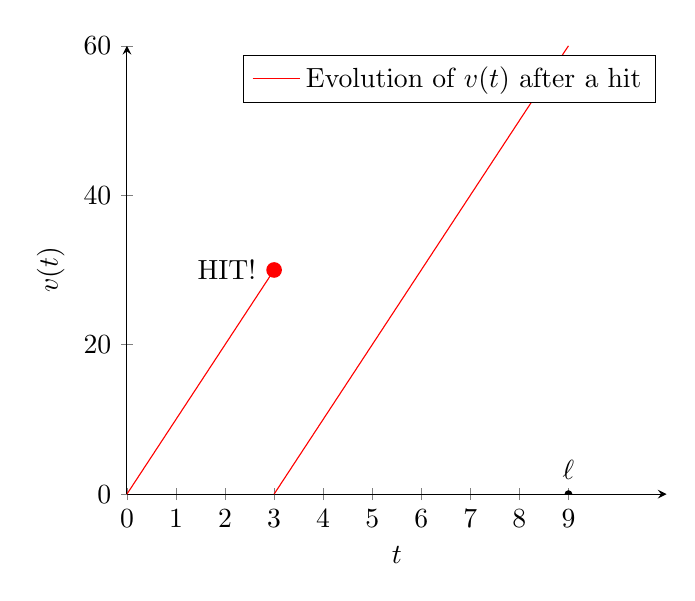
\begin{tikzpicture}
	\title{Evolution of electrons' speed after a hit}
	\begin{axis}[
	axis lines = left,
	xlabel = $t$,
	ylabel = {$v(t)$},
	xmin=0,
	xmax=11,
	xtick={0, 1,...,9},
	]
	%Below the red line is defined
	\addplot [
	domain=0:3, 
	samples=100, 
	color=red,
	]
	{10*x};
	\addlegendentry{Evolution of $v(t)$ after a hit}
	%Here the blue line is defined
	\addplot [
	domain=3:9,
	color=red,
	]
	{10*x -30};
	%\addlegendentry{after the first hit}
	
	\node[label={180:{HIT!}},circle,fill=red,inner sep=2pt] at (axis cs:3,30) {};
	\node[label={90:{$\ell$}},circle,fill,inner sep=1pt] at (axis cs:9,0) {};
	
	\end{axis}
	\end{tikzpicture}
\end{center}
In a difficult way, the average speed of the electrons can be expressed by the area underlying the red line divided by the total amount of time: $\bar{v}$ of function $v(t)$ is $\frac{1}{t_1}\int_{0}^{t_1} v(t) \cdot dt$.\\
In an easier way we can observe that between the $(i-1)^{th}$  and the $i^{th}$ hit $\bar{v_i} = \frac{h}{2} = \frac{a\cdot \Delta t}{2}$, and so $\bar{v} = \frac{\bar{h}}{n}= a \cdot \frac{\sum\Delta t}{n} = a \cdot \bar{t}$, where $n$ is the number of hits and $\bar{t}$ is the \I{average flying time}. 
By consequence
\begin{equation}
\bar{v} = a \cdot \bar{t} = \frac{\bar{t} \cdot q}{m}\cdot E = \mu_p \cdot E
\end{equation}  
\index{Carrier Mobility}
Where we introduce the \index{Electron mobility} \B{\I{Electron Mobility}} $\mu_p$, that depends on $\bar{t}$, which is a material constant.
\begin{equation}
\mu_p = \ [\frac{cm^2}{V \cdot s}]
\end{equation}  
Mobility is a constant even for \B{holes} and usually it is related to electron mobility by the law
\begin{equation}
\mu_p \sim 3\mu_n
\end{equation}
where $\mu_p$ is the \I{electron mobility} and $\mu_n$ is the \I{holes mobility} \index{Holes Mobility}. 
The fact that $\mu_p > \mu_n$ doesn't surprise ourself because \B{holes} move in \I{valence band}, which is normally fulfilled of carriers, while \B{electrons} move in \I{conductance band}, where the movement is less influenced by other carriers and by nuclei.  
\begin{center}
	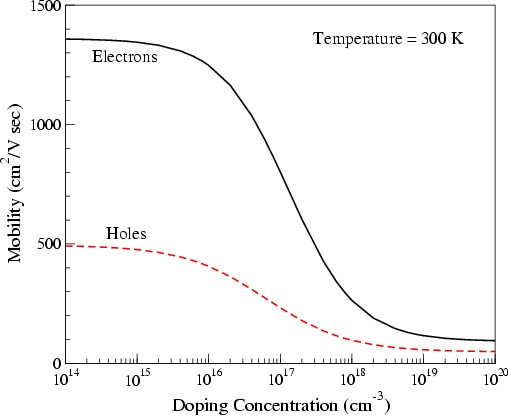
\includegraphics[width=7 cm]{mob.png}
	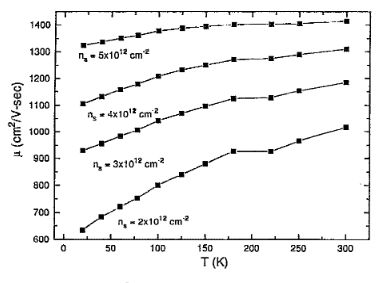
\includegraphics[width=7 cm]{mobilityT} %https://pdfs.semanticscholar.org/82da/3c040072ae6643613b8f93da170c976effea.pdf
	\\
	In the figure we can observe that mobility is negatively influenced by doping \index{doping} concentration, but positively by temperature.
	NOT TRUE, HAD TO BE REVIEWED \index{TO DO}
\end{center}

\subsubsection{Numerical analysis}
Given a bar with:
\begin{itemize}
	\item left-side potential = 0 V
	\item right-side potential = $+V$ (given by a generator)
	\item bar lenght $\ell$ and area $A$
\end{itemize}
\index{TO DO} Check for signs in equations
Being $V = -\int_{0}^{\ell}Ed\ell$ and assuming the electric field $E$ being constant in the bar, $V = -E\int_{0}^{\ell}d\ell = -E\cdot{\ell}$, so we can say $|E| = \frac{V}{\ell}$.\\
By definition,
\begin{equation}
I = \frac{\Delta Q}{t} = I_n + I_p
\end{equation} where $t$ is the transit-time and $I_n$, $I_p$ being relatively the current generated by negative carriers going to the right side of the bar (electrons) and by positive carriers going to the left side of the bar (holes). 
\subsubsection{$I_n$}
$I_n = \frac{q \cdot number \ of \ electrons}{t_{tr}}$. Being $number of electrons = n \cdot v$, where $n$ is the electrons concentration in the semiconductor bar $[\frac{electrons}{cm^3}]$ and $v= \ell \cdot A$ is the volume of the bar, we can write the following equation: $I_n = \frac{q \cdot n \cdot \ell A}{t_{tr}}$. Writing $t_{tr} = \frac{\ell}{v_n} = \frac{\ell}{\mu_p \cdot E}$ we finally can say that
\begin{equation} \label{eq:6}
\tcbhighmath[drop fuzzy shadow = green, colback = green!20!white, colframe = green]{
	I_n = \frac{q n \ell A}{\frac{\ell}{\mu_p \cdot E}} = \frac{q n \ell A}{\frac{\ell}{\mu_p \cdot \frac{V}{\ell}}}= \mu_n qn\frac{A}{\ell}\cdot V}
\end{equation}
We observe that \ref{eq:6} is the famous \B{Ohm's law} \index{Ohm's law}
\begin{equation}
R = \frac{1}{\mu_n q n}\frac{\ell}{A}
\end{equation}
where all the variables are related to the physical state of the bar.
\subsubsection{Resistivity and conductivity}
Doing a reasoning analogue to that for $I_n$, we can observe that $I_p = \mu_p qn\frac{A}{\ell}\cdot V$. The general expression of the current intensity in the bar is so given by:
\begin{equation}
I = (n\mu_n+p\mu_p)q\cdot \frac{\ell}{A} \cdot V
\end{equation}
\index{Resistivity}\index{Conductivity}
where the first term, $(n\mu_n+p\mu_p)q = \sigma $ is called \I{conductivity} of the material.\\
$\rho = \frac{1}{\sigma}$ is the resistivity of the material. 
Resistivity is a special characteristic of the material. 
\begin{equation}
\rho = [cm \cdot \Omega]
\end{equation}

\subsubsection{Diffusion Current} \index{Diffusion current}
The phenomenon of Diffusion Current is a characteristic of semiconductor materials. \\
When there is a nonuniform concentration of charge carriers (e.g. \I{holes}) we can 'sit' in a point (the point 0 in the figure) and observe that there is a \I{gradient} $\frac{dp}{dx}$ for the function $p$ to the left direction. The existence of this gradient implies that on the left of it the holes concentration is higher and on the right of it it will be lower. Imaging this point as a surface, it will be reasonably to think that there are more holes that will come from right to left than otherwise. So, we can assert that there is a statistical current (only due to this statistical observation) over the semiconductor called \B{Diffusion Current}. \\
The \I{Diffusion hole-current density} $J_p [\frac{A}{cm^2}]$ is proportional to the concentration gradient $\frac{dp}{dx}$ and is given by
\begin{equation}
J_p = -qD_p\frac{dp}{dx}
\end{equation}
where $D_p$ is called the \I{diffusion constant} for holes. The minus sign is necessary because the gradient is directed to the direction of maximum increment, so that $J_p$ will be positive for increments of $x$. 
\subsubsection{Total current}
Hence we can state that the total current over a doped semiconductor bar is given by:
\begin{equation}
I_{TOT} = I_p + I_n	
\end{equation}
where 
\begin{enumerate}
	\item $I_n$ = $q \mu_nn \frac{A}{L} V + q D_n \frac{dn}{dx}$
	\item $I_p = q \mu_pp \frac{A}{L} - q D_p \frac{dp}{dx}$
\end{enumerate}


Diffusion current is a current in a semiconductor caused by the change of concentration of carriers in a semiconductor. \\
\begin{center}
	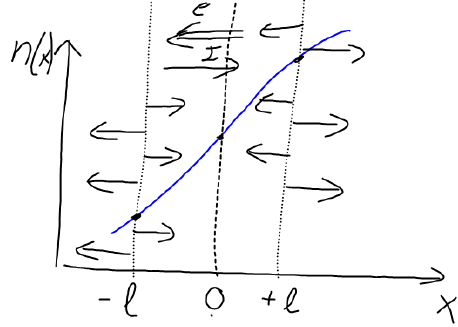
\includegraphics[width=7cm]{diffusion}
\end{center}

We can say, by an act of semi-religious acceptance, that the flux at point 0 is subjected to the law:
\begin{equation}
\Phi_e(0) = \frac{1}{2}n(+\ell)v_{TH}-\frac{1}{2}n(-\ell)v_{TH}
\end{equation}
And, at the end of some points that I can't get at this moment, we conclude that
\begin{equation}
I_{DIFF} = -qA\Phi_e= -(qv_{TH}\ell)A\frac{dn}{dx} = -qD_n\frac{dn}{dx}A
\end{equation}
Where $V_{TH}$ is the \I{thermal speed}, and $D_n$ is the \I{diffusion constant} of the electrons.

\section{Diodes}

Diodes are defined as $p-n$ junctions, that is by a boron-doped zone and a phosphorus-doped zone. We suppose that the two zones are aligned together with an \I{interface}. \\
We can observe, supposing a doping concentration of $10^{16}$:
\bite
	\item holes in p-zone = $10^{16}$
	\item electrons in p-zone = $n = \frac{i_n^2}{p} = 10^4$, which is a very little number compared to p.
	\item Vice-versa is valid for the n zone.
\fite
This gradient of charge carriers distribution make a flux to happen between the two zones of the diode, creating a third zone, the \B{Space charge region} in which electrons and holes recombine together and leave only positive or negative ions. This electron and holes movement is called \I{diffusion current}.The problem with this diffusion current is that, leaving the atom, charge carriers create ions, which generate an electric field that tries to bring that charge carriers back. 
\subsection{The equilibrium}
Once the equilibrium has been reached, we can observe that only a small region over the junction has been subjected to electron-holes annihilation. In this region there is an electric field  due to the presence of opposed sign charges between the junction. The natural tension creating over the junction is called \index{Built-in tension} \B{built-in tension} $V_{BI}$. A standard value for $V_{BI}$ is between 0.8/0.9 V.

\subsection{Formulas}
\bite 
	\item Direct-bias current:\index{Direct-bias current}
	\[ I_D = I_0(e^{\frac{V_d}{\frac{kT}{q}}}-1)\]
	\item Work current: \index{Work current} $I_D$ when $V_d = 0.7 V$.
	\[ I_0 = 10^{-15} A \rightarrow I_D = 10 \mu A \]
	\[   I_0 = 10^{-10} A \rightarrow I_D = 1 A.
	\]
	\item Inverse-bias current: \index{Inverse-bias current}
	\[I_D \simeq I_0\]
	\item NOTE THAT the true peak of 220V current is $220\sqrt{3} = 311 V$ 
\fite


In a $p-n$ junction there are three different "zones" based on ion characteristic:
\begin{enumerate}
	\item The p zone, with free holes and negative ions, is doped with Boron
	\item The n zone, with free electrons and positive ions, is doped with Phosphorus
	\item The \I{Space charge region}, the middle section of the diode, with thickness $ \simeq 0.5 \mu m$, where the free holes and free electrons got annihilated resulting in a zone with only negative (positive) ions on the left (right) part of this region. 
\end{enumerate}
In the \I{space charge region} there is a resulting electric field $\epsilon$ that prevent holes from the p-zone to annihilate with electrons from the n-zone. 
Under open circuited conditions, the net hole current must be zero, and so the diffusion current caused by the great amount of holes in the left part must be balanced by another flux, caused by the electric filed $\epsilon$. 
\[
	-qN_DV\frac{dp}{dn} = ?
\]




Diodes are defined as a p-n junction.
\begin{circuitikz}
	\draw (0,0) to[Do, l=$Diode$, i>^=$i$, v = $v$] (2,0);3
\end{circuitikz}
Is is made by two parts: the left part (according to the figure) is a p-doped semiconductor in which there are holes left.
The other part, on the contrary, is n-doped in which there are electrons left.

 

\newpage



\section{MOSFET}
The MOSFET (Metal Oxyde Semiconductor Field Effect) is a tripole composed by a MOS structure (from top to bottom: a metal, an oxide and a usually p-doped semiconductor).
\subsection{Functioning}
\bite
	\item When a positive potential is given to the metal terminal (called Gate) $V_G$, the minorities charge carriers (electrons) create a little film at the junction with the oxide. In this region takes place an \I{inversion}, because a lot of electrons are present even if the semiconductor is p-doped. In the oxide zone there is an electric Field.
	\item If a potential is applied to the Drain, a current is possible within the inversion zone. The different doping of source and drain an the n-nature of the inversion zone prevent current to flow into the semiconductor: this difference act like an inverse-bias diode. 
\fite
Note that the current starts flowing when the concentration of electrons is equal to the standard holes concentration of the semiconductor. 

\subsection{Pinch-off and saturation}
When $V_D = V_T$ we have that the gate tension is not sufficient to 


\section{FORMULAS}
\subsection{Electric field and semiconductors}

Electrostatic force between two charges $q_1 q_2$ at a distance $r$: \index{Electromagnetic Force} \begin{equation}
	F = \frac{1}{4\pi\epsilon_0}\frac{q_1q_2}{r^2}
\end{equation} \\ 
\index{Electric Field} The Electric field (as the force which a charge $q$ is subjected to in a point of the space divided by the charge $q$)
	\begin{equation}
		E = \frac{F}{q} = \frac{1}{4\pi\epsilon_0}\frac{Q}{r^2}
	\end{equation} Note that the Electric field is a \B{CONSERVATIVE FIELD}\\
\index{Conservative field} 
	A conservative field is a field in which the \I{Work} done for placing an element from a point $a$ to a point $b$ depends only from the different location of $a$ and $b$ and not by the route done.\\

\index{Work} The \I{Work} in a conservative field is defined as follows:
		\begin{equation}
			W_{a\to b} = \int_{a}^{b} \overrightarrow{F}(x)dx = q (V_b - V_a)d
		\end{equation}\\
\index{Potential Energy} The \I{Potential energy} of a charge subjected to an Electric field is 
	\begin{equation}
		U = q V [eV]
	\end{equation} and the measure unit is the electronVolt $eV$, where $1 eV = 1,6 \ 10^{-19} J$, the energy necessary to move an electron from a point $a$ to a point $b$ with $V_a-V_b= 1 V$.

\index{Electric Potential}The \I{Electric Potential} at a point $r$ in an Electric Field $E$ is given by 
	\begin{equation}
		V_E = -\int_{C}E \cdot \mathrm{d} \boldsymbol{\ell}
	\end{equation}
	Where $C$ is an arbitrary path from the point $r$ to the point with zero potential. \\

\index{Electric Current} The \I{Electric Current} is defined as $i$ (from the french \I{intensité du courant}):
	\begin{equation}
		I = \frac{Q}{t} = \frac{V}{R} \ \ \ \ \ [Amp]
	\end{equation}
\index{Mass action Law} The \I{Law of mass action} is a relation about the concentration of free electrons and free holes in a semiconductor under thermal equilibrium. It states that the product of the concentration of free electrons and free holes is constant
\begin{equation}
	p\cdot n = n_i^2
\end{equation}
Where $n_i$, \I{intrinsic concentration}, is the concentration of electrons (or hole, that is the same) of a \I{pure} semiconductor.
\index{Question} Question: $i_n$ isn't a properly constant value: it depends on temperature and material (?)\\
\index{Discharge of the condenser} The \I{Discharge of the condenser} is an exponential process.
\begin{center}
\begin{circuitikz}[scale=1.2]\draw
	(0,0) node[ground] {}
	to[V=$V_Psin(\omega t)$] (0,2)
	to[diode={name=D}, *-*] (2,2)
	to[C] (2,0)
	(2,0)--(3,0)
	to[R, v=$V_{OUT}$] (3,2)
	(3,0) -- (0,0)
	(3,2) -- (0,2);
\end{circuitikz}
\end{center}
During the discharge of the condenser we have 
\[
	V_{OUT} = V_p e^{-\frac{t}{RC}}
\]





\newpage
\section{Engineer's corner}
\subsection*{Question 1: How much is $1 C$?} \index{Coulomb}
At first attempt we can say that 1 $Coulomb$ is \I{very} approximately $10^{19}$ times the fundamental charge unit (the electron). However it is a bit difficult rendering the idea of $10^{19}$ electrons. \\
Thinking about batteries, a common \I{AAA} battery has a capacity of 540 $mAh$, which are equivalent to 1944 $C$. \\
A common \I{AA} battery has a charge of 9 $kC$. \\
In everyday terms, a Coulomb is $\frac{1}{2000}$ times the charge occurring to empty a normal AAA battery.


\newpage
\section{Millman's questions}

\subsection*{Chapter 2}
\begin{itemize}
	\item[2.2] \B{Define mobility and give its dimension}\\ 
	\index{Mobility}Mobility is defined as the coefficient between the Electric field applied to a bar and the speed of charge carriers moving into the bar. Hence we can say $\mu = \frac{\bar v}{E} = [\frac{cm^2}{E}]$, it is usually described with non SI dimension $\frac{cm^2}{E}$.
	\item[2.3] \B{Define conductivity and give its dimension}\\ 
	\index{Conductivity} Conductivity is a material constant used to determine the resistance of a semiconductor. It is defined as $\sigma = (n\mu_n + p\mu_p)q$ and depends on doping. Its dimension are $[\frac{1}{\Omega \cdot m} = \frac{S}{m}]$ because it can also be expressed as $\sigma = \frac{1}{\rho} = \frac{\ell}{R\cdot A}$
	\item[2.4] \B{Define a hole (in a semiconductor)}\\ 
	A hole is the positive charge generated by the migration of an electron from an atom to another, leaving the first atom positively charged and neutralizing the second. In a general approach we can consider the holes mobility as a proper current. 
	\item[2.6] \B{Define intrinsic concentration of holes}\\
	\index{Intrinsic concentration} intrinsic concentration of holes is a coefficient $n_i$ temperature dependent that indicates the amount of free electrons (or holes, that is the same) in a pure semiconductor. The relation between the intrinsic concentration of holes and the holes density is given by the following $n_i^2 = n \cdot p$. At $0^o K, n_i = 0$. This fact has two explanation: the first is that at the absolute zero no energy is given to the electrons from the outside, hence it is impossible to break the covalent bonds between atoms. The second is based on the expression of $n_i$: $n_i \propto \epsilon^{-\frac{1}{T}}$, so the limit for this function for $T\rightarrow0 = 0$. 
	\item[2.9] \B{Define donor and acceptors impurities}\\ 
	\index{Donor}\index{Acceptor}A semiconductor can be doped by donors (acceptors) atoms from the IV (III) group, like Phosphorus (Boron). These atoms, called impurities, fit in the lattice structure and tend to donate (accept) an electron, due to their atomic structure. In fact, Phosphorus (Boron) atoms reach their stability with 3 (5) electrons. 
	\item[2.2] \B{A semiconductor is doped with both donors and acceptors of concentration $N_D$ and $N_A$ respectively. Write the equation from which to determine the electron and hole concentrations (n and p)}\\
	The equation ruling these relations are 
	\[
{n \cdot p = n_i^2}, {N_p + p = N_n + n}
	\]
	\item[2.14] \B{Given an intrinsic semiconductor specimen, state two physical processes for increasing its conductivity and explain briefly}\\ 
	The conductivity is defined as $\sigma = q (n\mu_p + p\mu_p)$. We can alter $\sigma$ by altering $n$ or $p$. This can be done in two ways:
	\begin{enumerate}
		\item Doping the semiconductor, and so altering directly $n$ and $p$
		\item Heating the semiconductor will result in a change in $n_i^2$: knowing that $n_i^2 = n \cdot p$ this will result in an increase of either of them.
	\end{enumerate}
	\item[2.15] \B{Is the \I{temperature coefficient of resistance} of a semiconductor positive or negative?}\\ 
	We know that heating the semiconductor will result in a reduction of its resistance, so the \I{temperature coefficient of resistance} is reasonably negative. On the contrary, for a metal heating process increases resistance, hence we can assert that for a metal the \I{temperature coefficient of resistance} is a positive quantity. 
	\item[2.22] \B{Define \I{Diffusion constant for holes}, for electrons and give their dimensions}\\
	The \I{Diffusion constant} is a constant associated to the \I{diffusion current}, a phenomenon that occurs when it exists a gradient in holes (electron) density. Being $J_S = -qN_D\frac{dp}{dx}$ we observe that $N_D = \frac{J_S}{q \cdot\frac{dp}{dx}} = [\frac{A}{C \cdot cm^{-3}}]= [\frac{A \cdot cm^3}{C}]$.
\end{itemize}
\subsection*{Chapter 3}
\begin{enumerate}
	\item[3.2] \B{What is the order of magnitude of the space-charge width at a \I{p-n junction}? What does this space charge consist of (electrons, holes, ions, neutral acceptors......)?}\\
	The space-charge width similar equally to the wavelength of visible light, $5 \mu m$. This space-charge region consist in a junction between p and n doped section of a semiconductor in which the holes of the n section are 'filled' by the electrons from the p section. In this region there is an electric field which intensity is similar to 0.8/0.9 V usually. 
	\item[3.2] \B{For a reverse-biased diode, does the transition region increase or decreas in width? What happens to the junction potential?}\\
	For a reverse-biased diode, the transition region enlarges, this making more difficult for secondary carriers to travel from one edge to another. This result is generally approximated by an absence of electric current, even if a very light current (usually of the magnitude oder of $nA$) is flowing. 
		 
\end{enumerate}



% --------------------------------------------------------------
%                         Sample structures
% --------------------------------------------------------------


\newpage
%Below is an example of the problem environment
\begin{problem}{6}
\begin{enumerate}[label=\alph*)]
    \item Suppose an entire function $f$ is bounded by $M$ along $|z|=R$. Show that the coefficients $C_k$ in its power series expansion about $0$ satisfy
    \[
    |C_k|\leq\frac{M}{R^k}.
    \]
    \item Suppose a polynomial is bounded by $1$ in the unit disc. Show that all its coefficients are bounded by 1.
\end{enumerate}
\end{problem}

%Below is the solution environment
\begin{solution}{}
Part a): Since $f$ is an entire function it can be expressed as an infinite power series, i.e.
\[
f(z)=\sum_{k=0}^\infty\frac{f^{(k)}(0)}{k!}z^k=\sum_{k=0}^\infty C_kz^k.
\]
If we recall Cauchy's Integral we have
\[
f(z)=\frac{1}{2\pi i}\int_\gamma\frac{f(w)}{w-z}\ dw,
\]
carefully notice that $\frac{1}{w-z}=\frac{1}{w}\cdot\frac{1}{1-\frac{z}{w}}$ can be written as a geometric series. We have

%The align environment with no label
\begin{align*}
\frac{1}{2\pi i}\int_\gamma\frac{f(w)}{w-z}\ dw &=\frac{1}{2\pi i}\int_\gamma\left\lbrace\frac{f(w)}{w}\cdot\left(\frac{1}{1-\frac{z}{w}}\right) \right\rbrace\ dw\\[8pt]
&=\frac{1}{2\pi i}\int_\gamma\left\lbrace\frac{f(w)}{w}\cdot\left(1+\frac{z}{w}+\frac{z^2}{w^2}+\frac{z^3}{w^3}+\cdots\right) \right\rbrace\ dw\\[8pt]
&=\left(\frac{1}{2\pi i}\int_\gamma \frac{f(w)}{w}\ dw\right)z^0+\left(\frac{1}{2\pi i}\int_\gamma \frac{f(w)}{w^2}\ dw\right)z^1+\left(\frac{1}{2\pi i}\int_\gamma \frac{f(w)}{w^3}\ dw\right)z^2\cdots
\end{align*}
Now take the modulus of $C_k$ to get
\[
|C_k|=\left\lvert\frac{1}{2\pi i}\int_\gamma \frac{f(w)}{w^{k+1}}\ dw \right\rvert\leq\frac{1}{2\pi}\int_\gamma\frac{|f(w)|}{|w^{k+1}|}\ |dw|\leq \frac{M}{2\pi}\int_\gamma\frac{|dw|}{|w^{k+1}|}
\]
Then integrate along $\gamma(\theta)=Re^{i\theta}$ for $\theta\in [0,2\pi]$ to get
\[
|C_k|\leq \frac{M}{2\pi}\int_0^{2\pi}\frac{|iRe^{i\theta}\ d\theta|}{|R^{k+1}e^{ik\theta}|}=\frac{M}{2\pi\cdot R^k}\int_0^{2\pi}\ d\theta=\frac{M}{R^k}.
\]
Hence, $|C_k|\leq \frac{M}{R^k}$.
\end{solution}
\pagebreak



\printindex

\end{document}
